\documentclass[a4paper]{article}

\usepackage[utf8]{inputenc}
\usepackage[DIV=20]{typearea}
\usepackage{microtype}
\usepackage{mathtools, amssymb, bm}
\DeclareMathOperator*{\argmax}{arg\,max}
\DeclareMathOperator*{\argmin}{arg\,min}
\renewcommand{\P}{\textsf{Prob}}
\usepackage{parskip}
\usepackage{subcaption}
\usepackage{float}
\usepackage[shortlabels]{enumitem}
\usepackage[colorlinks=true]{hyperref}
\hypersetup{linktoc=all}

\title{5}
\date{}

\begin{document}
\maketitle
\section{MAP Estimation}
We know that $\bm{y}=\bm{\Phi}\bm{x}+\bm{\eta}$ where $\bm{x}\in\mathbb{R}^n,\bm{y},\bm{\eta}\in\mathbb{R}^m, \bm{\Phi}\in\mathbb{R}^{m\times n}$. Also, $\bm{x}\sim \mathcal{N}(0,\bm{\Sigma}_{\bm{x}}), \bm{\eta}\sim \mathcal{N}(0,\sigma^2\bm{I}_{m\times m})$

Now, the MAP estimate for $\bm{x}$ is given by
\begin{align*}
\bm{\hat{x}}
&= \argmax_{\bm{x}} \P(\bm{x} | \bm{y})\\
&= \argmax_{\bm{x}} \frac{\P(\bm{y} | \bm{x}) \P(\bm{x})}{\P(\bm{y})} & \text{(Bayes' rule)}\\
&= \argmax_{\bm{x}} \P(\bm{y} | \bm{x}) \P(\bm{x}) & \text{(as $\P(\bm{y})$ is a constant)}\\
&= \argmax_{\bm{x}} \underbrace{\frac{1}{(2\pi\sigma^2)^{m/2}}\exp{-\frac{\|\bm{y}-\bm{\Phi}\bm{x}\|_2^2}{2\sigma^2}}}_{\P(\bm{y} | \bm{x})} \underbrace{\frac{1}{(2\pi)^{n/2}|\bm{\Sigma}_{\bm{x}}|^{1/2}}\exp{-\frac{\bm{x}^T\bm{\Sigma}_{\bm{x}}^{-1}\bm{x}}{2}}}_{\P(\bm{x})}\\
&= \argmax_{\bm{x}} \exp{-\frac{\|\bm{y}-\bm{\Phi}\bm{x}\|_2^2}{2\sigma^2}} \exp{-\frac{\bm{x}^T\bm{\Sigma}_{\bm{x}}^{-1}\bm{x}}{2}} & \text{(ignoring scaling constants)}\\
&= \argmin_{\bm{x}} \frac{\|\bm{y}-\bm{\Phi}\bm{x}\|_2^2}{2\sigma^2} + \frac{\bm{x}^T\bm{\Sigma}_{\bm{x}}^{-1}\bm{x}}{2} & \text{(taking negative logarithm)}\\
&= \argmin_{\bm{x}} \frac{(\bm{y}-\bm{\Phi}\bm{x})^T(\bm{y}-\bm{\Phi}\bm{x})}{2\sigma^2} + \frac{\bm{x}^T\bm{\Sigma}_{\bm{x}}^{-1}\bm{x}}{2}\\
&= \argmin_{\bm{x}} \frac{\bm{y}^T\bm{y}-(\bm{\Phi}\bm{x})^T\bm{y}-\bm{y}^T\bm{\Phi}\bm{x}+(\bm{\Phi}\bm{x})^T\bm{\Phi}\bm{x}}{2\sigma^2} + \frac{\bm{x}^T\bm{\Sigma}_{\bm{x}}^{-1}\bm{x}}{2}\\
&= \argmin_{\bm{x}} \underbrace{\frac{-\bm{x}^T\bm{\Phi}^T\bm{y}-\bm{y}^T\bm{\Phi}\bm{x}+\bm{x}^T\bm{\Phi}^T\bm{\Phi}\bm{x}}{2\sigma^2} + \frac{\bm{x}^T\bm{\Sigma}_{\bm{x}}^{-1}\bm{x}}{2}}_{=\bm{F} \text{ (let)}} & \text{(ignoring additive constants)}\\
\end{align*}
Now, to optimise $\bm{F}$, set $\dfrac{\,\textrm{d}\bm{F}}{\,\textrm{d}\bm{x}} = 0$
\begin{align*}
\dfrac{\,\textrm{d}\bm{F}}{\,\textrm{d}\bm{x}}
&= \frac{\,\textrm{d}}{\,\textrm{d} \bm{x}}\left(\frac{-\bm{x}^T\bm{\Phi}^T\bm{y}-\bm{y}^T\bm{\Phi}\bm{x}+\bm{x}^T\bm{\Phi}^T\bm{\Phi}\bm{x}}{2\sigma^2} + \frac{\bm{x}^T\bm{\Sigma}_{\bm{x}}^{-1}\bm{x}}{2}\right)\\
&= \frac{\,\textrm{d}}{\,\textrm{d} \bm{x}}\left(\frac{-\bm{x}^T\bm{\Phi}^T\bm{y}}{2\sigma^2}\right) + \frac{\,\textrm{d}}{\,\textrm{d} \bm{x}}\left(\frac{-\bm{y}^T\bm{\Phi}\bm{x}}{2\sigma^2}\right) + \frac{\,\textrm{d}}{\,\textrm{d} \bm{x}}\left(\frac{\bm{x}^T\bm{\Phi}^T\bm{\Phi}\bm{x}}{2\sigma^2}\right) +  \frac{\,\textrm{d}}{\,\textrm{d} \bm{x}}\left(\frac{\bm{x}^T\bm{\Sigma}_{\bm{x}}^{-1}\bm{x}}{2}\right)\\
&= \left(\frac{-\bm{\Phi}^T\bm{y}}{2\sigma^2}\right) + \left(\frac{-(\bm{y}^T\bm{\Phi})^T}{2\sigma^2}\right) + \left(\frac{\left(\bm{\Phi}^T\bm{\Phi}+(\bm{\Phi}^T\bm{\Phi})^T\right)\bm{x}}{2\sigma^2}\right) +  \left(\frac{\left(\bm{\Sigma}_{\bm{x}}^{-1}+(\bm{\Sigma}_{\bm{x}}^{-1})^T\right)\bm{x}}{2}\right)\\
&=\left(\frac{-2\bm{\Phi}^T\bm{y}}{2\sigma^2}\right) + \left(\frac{2\bm{\Phi}^T\bm{\Phi}\bm{x}}{2\sigma^2}\right) +  \left(\frac{2\bm{\Sigma}_{\bm{x}}^{-1}\bm{x}}{2}\right)\\
&\Rightarrow \left(\frac{-\bm{\Phi}^T\bm{y}+\bm{\Phi}^T\bm{\Phi}\bm{x}}{\sigma^2}\right) + \bm{\Sigma}_{\bm{x}}^{-1}\bm{x}=0\\
&\Rightarrow -\bm{\Phi}^T\bm{y}+\bm{\Phi}^T\bm{\Phi}\bm{x} + \sigma^2\bm{\Sigma}_{\bm{x}}^{-1}\bm{x}=0\\
&\Rightarrow \left(\bm{\Phi}^T\bm{\Phi} + \sigma^2\bm{\Sigma}_{\bm{x}}^{-1}\right)\bm{x} = \bm{\Phi}^T\bm{y}\\
&\Rightarrow \bm{x} = \left(\bm{\Phi}^T\bm{\Phi} + \sigma^2\bm{\Sigma}_{\bm{x}}^{-1}\right)^{-1}\bm{\Phi}^T\bm{y}\\
\end{align*}
Hence, the MAP estimate of $\bm{x}$ is $\bm{\hat{x}} = \left(\bm{\Phi}^T\bm{\Phi} + \sigma^2\bm{\Sigma}_{\bm{x}}^{-1}\right)^{-1}\bm{\Phi}^T\bm{y}$.
% Now, to optimise $\bm{F}$, set $\frac{\d \bm{F}}{\d \bm{x}} = 0$
% \begin{align*}
% \frac{\d \bm{F}}{\d \bm{x}} 
% &= \frac{(\bm{y}-\bm{\Phi}\bm{x})^T\bm{y}-\bm{\Phi}\bm{x}}{2\sigma^2} + \\
% \end{align*}
\section{Observations}
\begin{figure}[H]
	\centering
	\begin{subfigure}{0.45\linewidth}
		\centering
		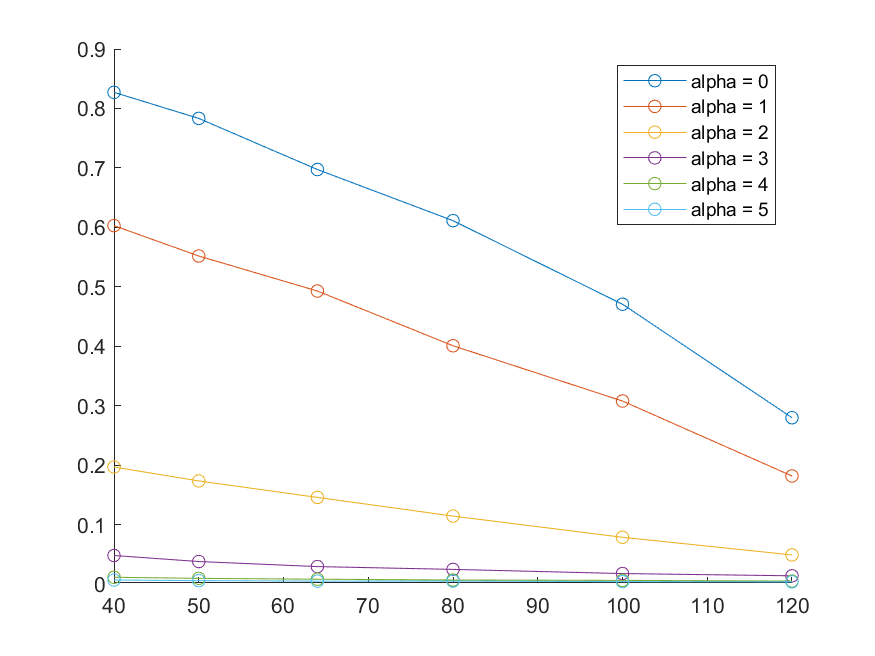
\includegraphics[width=\linewidth]{../media/Q5 RMSEs.png}
		\caption{}
	\end{subfigure}
	\begin{subfigure}{0.45\linewidth}
		\centering
		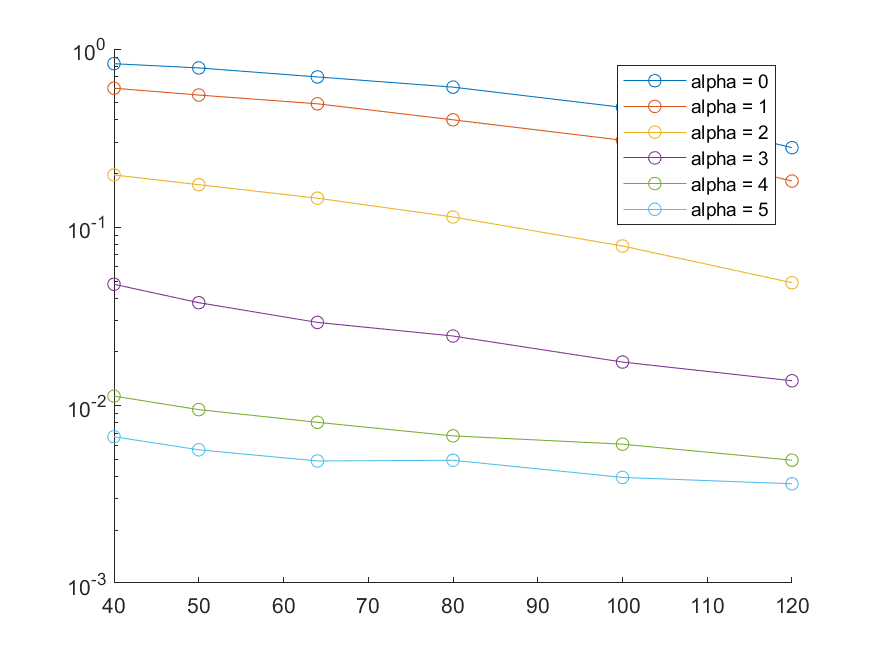
\includegraphics[width=\linewidth]{../media/Q5 RMSEs log Y-axis.png}
		\caption{$y-$axis on log scale}
	\end{subfigure}
	\caption{RMSE vs $m$ with varying $\alpha$}
\end{figure}
\begin{itemize}
\item RMSE is lower for higher $\alpha$ (more apparant on the log-scale)
\item RMSE is lower (or very close) as $m$ increases for a fixed $\alpha$
\item RMSE with $\alpha=3$ is $<0.05$ for all $m$ whereas RMSE ranges from $0.8271$ to $0.2797$ with $\alpha=0$
\end{itemize}
The reconstruction is better (lower RMSE) as $\alpha$ increases as the case of the convariance matrix with decaying eigenvalues is equivalent to signal sparsity in some orthonormal basis \emph{(slide 84 of Statistics of Natural Images)}
\end{document}